\chapter{研究背景}
\label{chap:haikei}

本章では手書きメモ・イラストを扱う既存のシステムの現状と、その問題点を整理する。

\newpage

\section{手書きのメモ・イラスト}
手書きによってメモやイラストを表現するのは、鉛筆等の筆記具と紙さえあればすぐに記録でき、また美麗な作品を描くことを目的としなければ、
特別な技量も要求されないため、情報を記録・表現する手法として広く普及している。
計算機の登場によりテキスト編集支援機能が充実したため、文章のみで完結する内容であれば手書きではなくタイピングによって記録するように置き換わったが、
アイデアのような文章のみでは表現しづらい構造を持った概念を表現する場合は文字と図を自在に混合させて配置できる手書きメモの方が適している。
また、テキストによってメモをとる場合はキーボードのような専用のハードウェアや、それらを使いこなすタッチタイピング等の技量が必要であるという問題点があるが、
手書きの場合は紙やペン等の筆記具が扱えれば良いため、ハードウェアや技能を必要とするテキスト入力と比較してより多くの人々が利用できる手段であると言える。

\section{タッチ・ペンインターフェースの普及}

\begin{figure}[htbp] \begin{minipage}{0.5\hsize}
                         \begin{center} {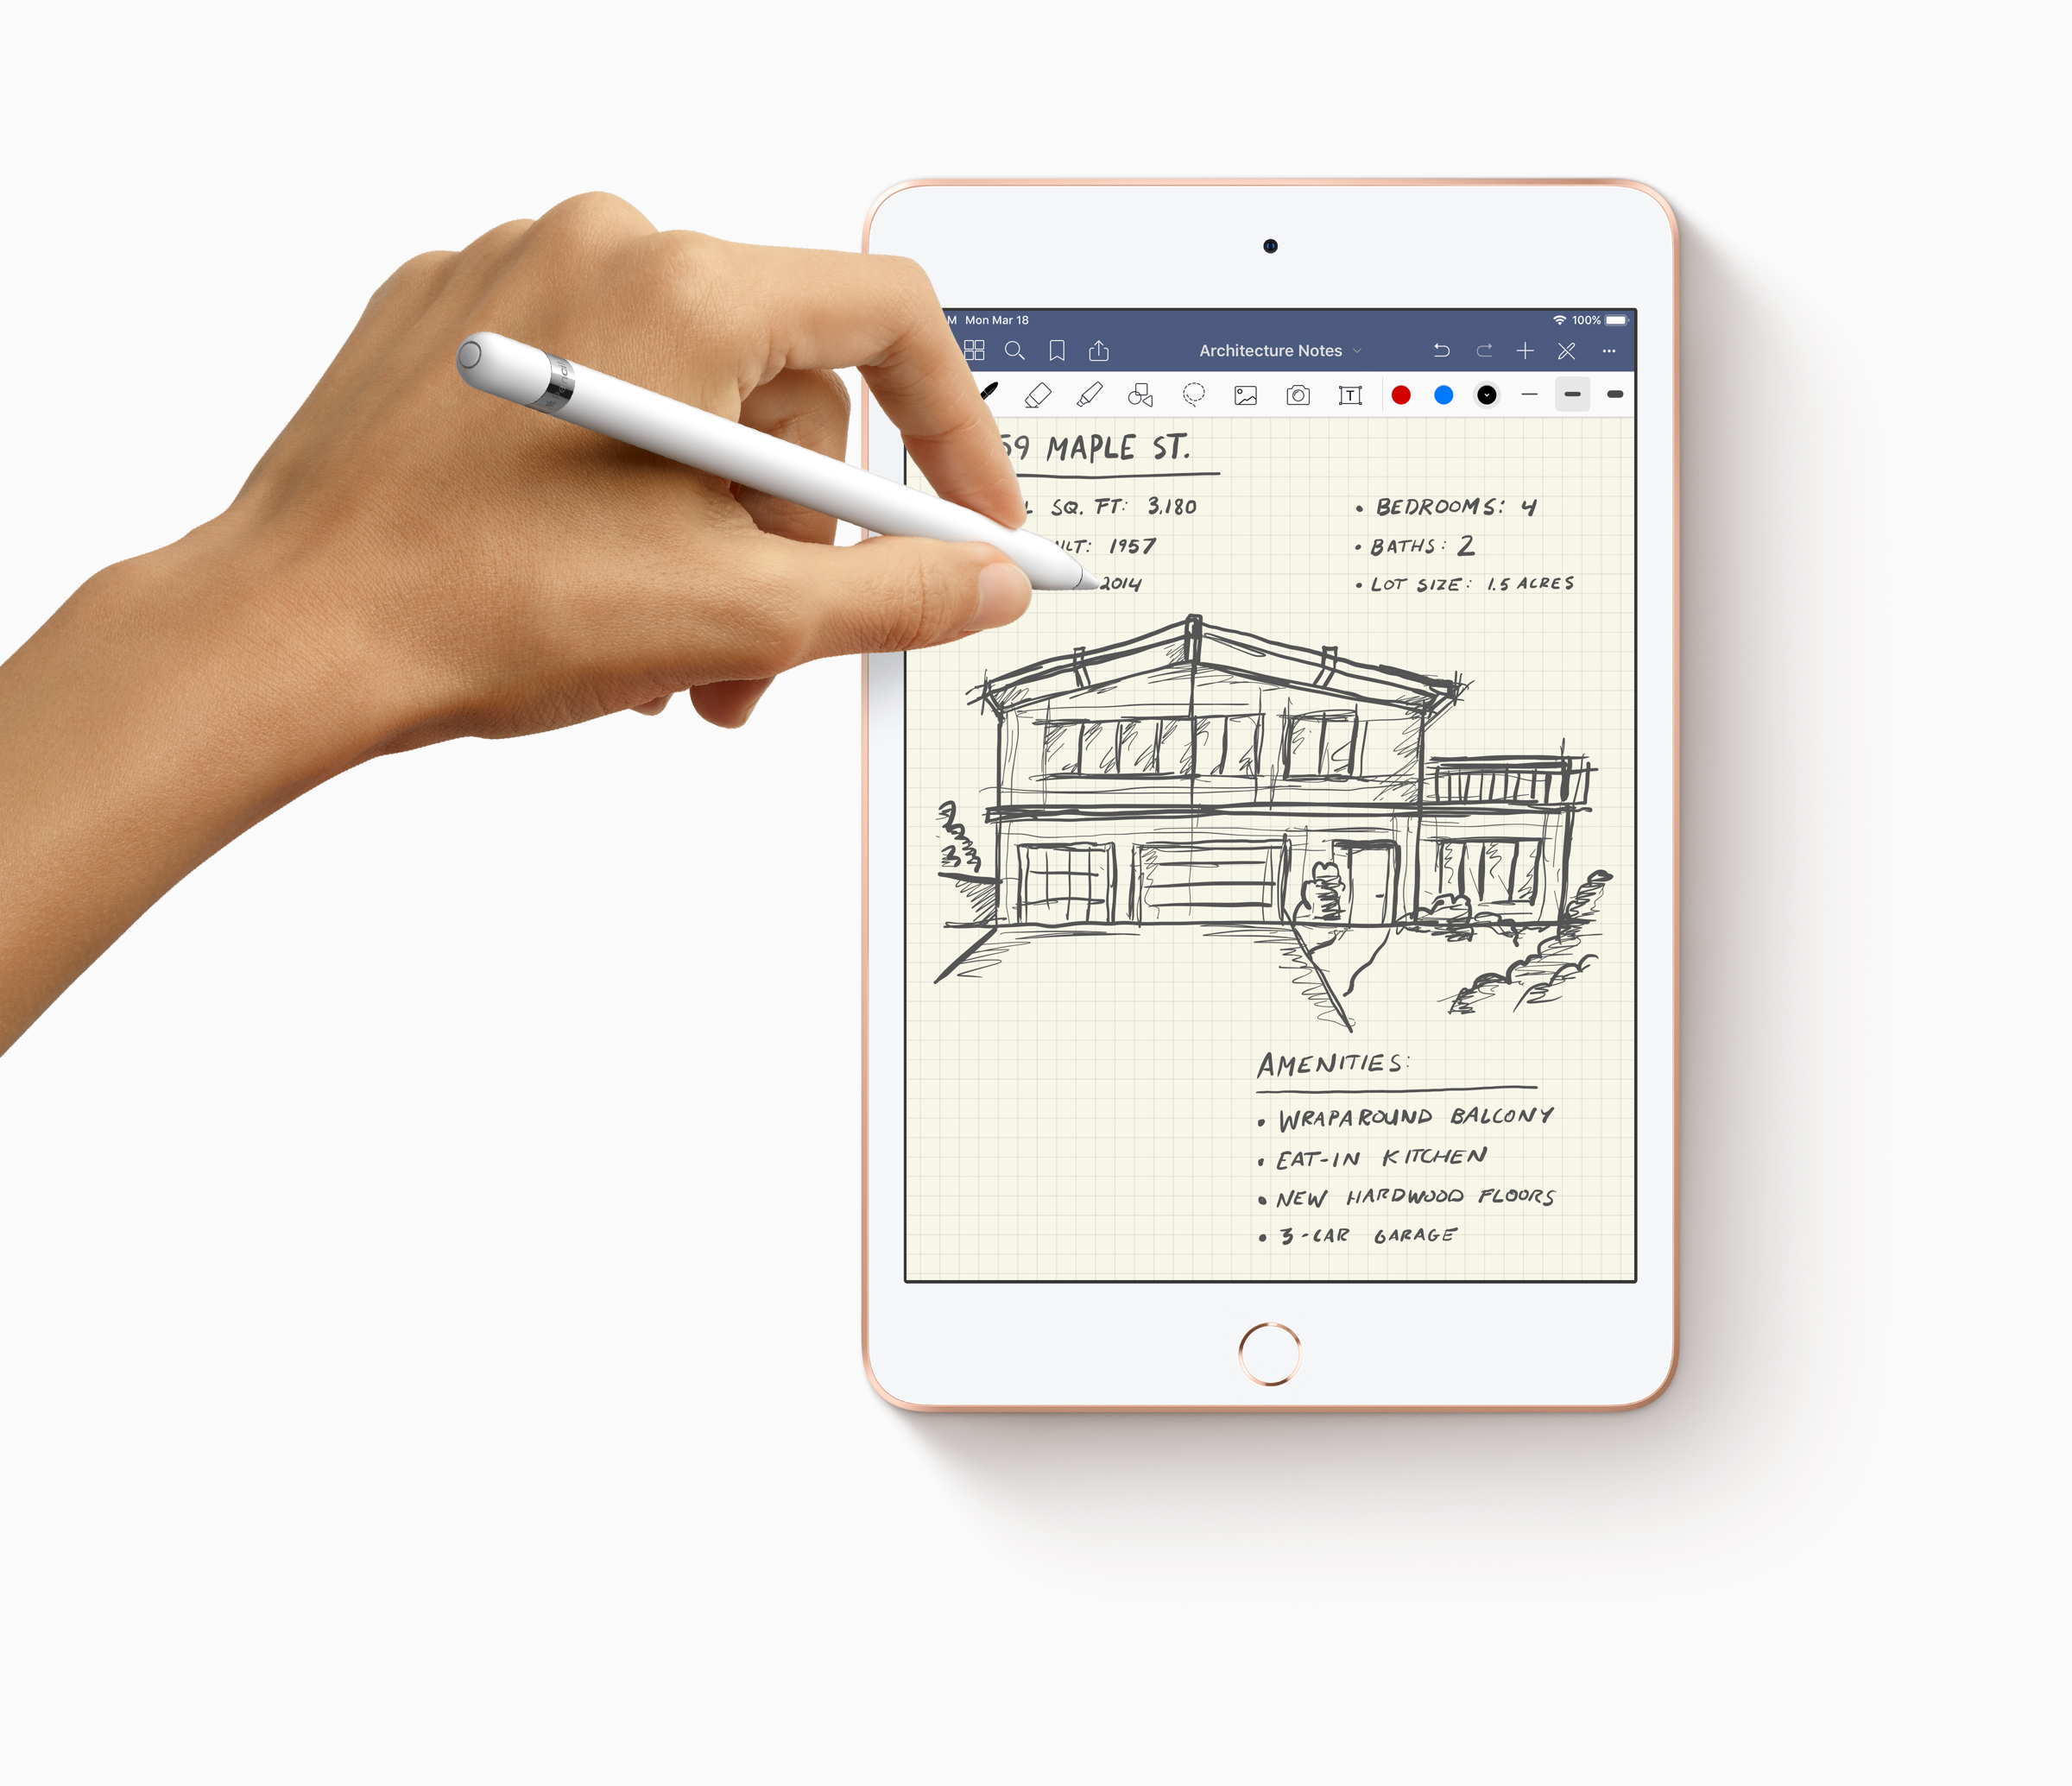
\includegraphics[width=40mm]{images/ipadmini.jpg}}
                         \end{center} \caption{iPad}
\end{minipage} \begin{minipage}{0.5\hsize}
                   \begin{center} {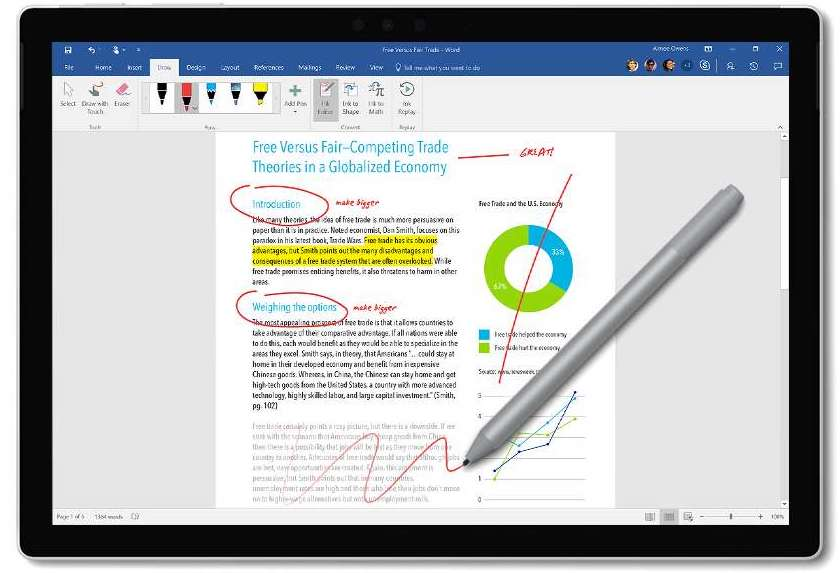
\includegraphics[width=40mm]{images/surface.jpg}}
                   \end{center} \caption{Surface}
\end{minipage}
\end{figure}

かつてはノートやスケッチブック等の紙の上で記録されていた手書きメモだが、タッチパネルやスタイラスペン等のインターフェースを備えたデバイスの普及に伴い、
計算機上で手書きメモを取ることが一般化してきた。
手書きメモやイラストを計算機の上で描く場合、マウスやトラックパッド等のポインティングデバイスではなく、
ペンインターフェースが好ましいとされるが、iOS\footnote{https://www.apple.com/jp/ios/}やWindows\footnote{https://www.microsoft.com/ja-jp/windows}、
ChromeOS\footnote{https://www.google.com/chromebook/}等の主要なプラットフォームで
スタイラスペンを備えた機種が充実しているため手書きでメモやイラストを描く環境は充分に整っている。